\section{Evaluation}
\label{section:evaluation}

%\begin{enumerate}
%	\item Evaluierung interessanter Aspekte anhand von Statistiken
%\end{enumerate}

When performing fully automated fuzzing, the full fuzzing process for one message takes around 5.5 seconds. The majority of time is consumed by the processing of the message on the constrained device. \Autoref{figure:fuzzing_performance} displays the processing time of a CoAP message with a different number of options in the header by the constrained devices. It shows the time that the different steps of the fuzzing process took. The maximum number of options is 19, which are all options that the Contiki-NG CoAP implementation knows. For each number of options, the average times of 130 messages were taken. When one option is used instead of no options, the processing time of the message increases a quarter of a second. This impact is very small compared to the increase of nearly three seconds, when using more than two options. A further increase of the number of options does not change the time it takes the constrained device to process the message. These results could imply that the processing of a single option is somehow optimized in Contiki-NG. But since we want to fuzz more than just one option at a time, we are stuck with the very poor performance of 5.5 seconds per message.

% This time can highly vary and depends heavily on the number given options in the CoAP message.
Setup times for the devices can vary due to cached binaries but can reach the magnitude of several minutes.

\begin{figure}[h]
	\centering
	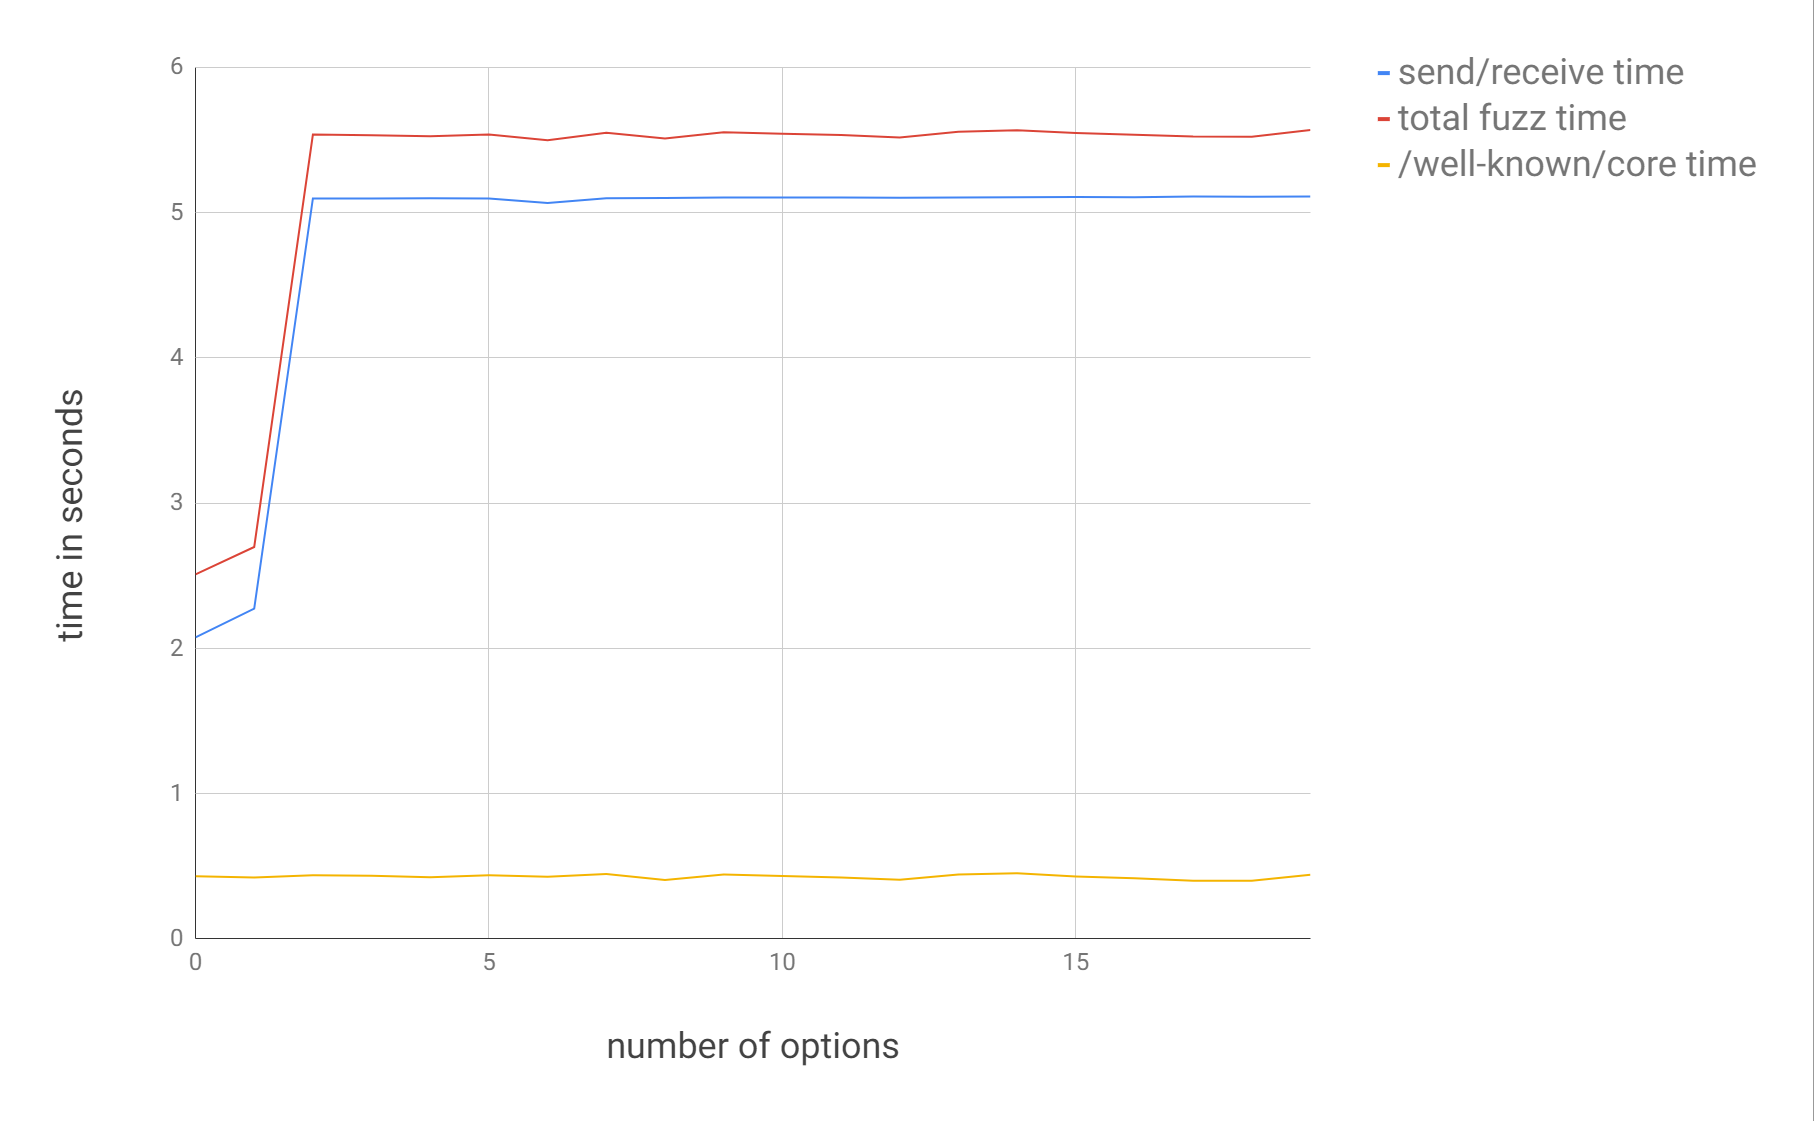
\includegraphics[width=0.5\textwidth]{images/fuzzing_performance}
	\caption{Processing time of CoAP messages with different amounts of options}
	\label{figure:fuzzing_performance}
\end{figure}

In order to evaluate the fuzzer and the system under test, we performed 60.000 fuzzing requests but did not succeeded in causing a crash or a device malfunction. In order to make sure that potential crashes can be found by our setup, we temporarily added an infinite loop to the CoAP implementation of Contiki-NG. This loop was entered if the token length had a specific value and the hardware watchdog subsequently triggered a restart. All of these expected crashes were properly tracked by our fuzzer.